% Chapter Template

\chapter{Dataset} % Main chapter title

\label{ch:04} % Change X to a consecutive number; for referencing this chapter elsewhere, use \ref{ChapterX}

%----------------------------------------------------------------------------------------
%	SECTION 1
%----------------------------------------------------------------------------------------

\section{Synthetic Dataset}
To train a deep learning model with supervised learning scheme, a dataset should require two principles, truth-worthy ground-truth and comprehensive scenarios. The depth map captured by Kinect is not satisfied the first requirement since it is usually semi-dense with a number of missing pixels, as shown in Figure \ref{fig:kinect-depth}. Therefore, a more elaborate depth map is required for the training work. In this thesis, a dataset called ``synthetic50-5" is created for the training works.


\subsection{Resource}
\cite{data1}, \cite{data2}, \cite{data3} and \cite{data4} published a set of point cloud dataset on the internet for computer vision task research. These point clouds are scanned from real objects using high resolution scanners like Cyberware 3030 MS+ and calibrated with post processing. Each objects has been scanned for hundreds of times for an exhaustive completion for the origin objects, which is up to millions points. (\cite{data1}). The dense point clouds makes the normal inference task trivial since the neighbor based method performs good enough for these kind of task. Some of the point cloud even equipped with pre-computed normal map based on more advanced methods. They all provides the accurate ground-truth for the supervised learning method.

The ``synthetic50-5", is a datset with 50 point clouds as training set and 5 point clouds as test set. The dataset is created base on the work of this thesis and using for normal inference task. Figure \ref{fig:dataset-demo} gives the illustrations of some objects. Appendix \ref{AppendixA} gives a full version of dataset models.

\begin{figure}[!h]
	\centering
	\begin{subfigure}[b]{0.23\linewidth}
		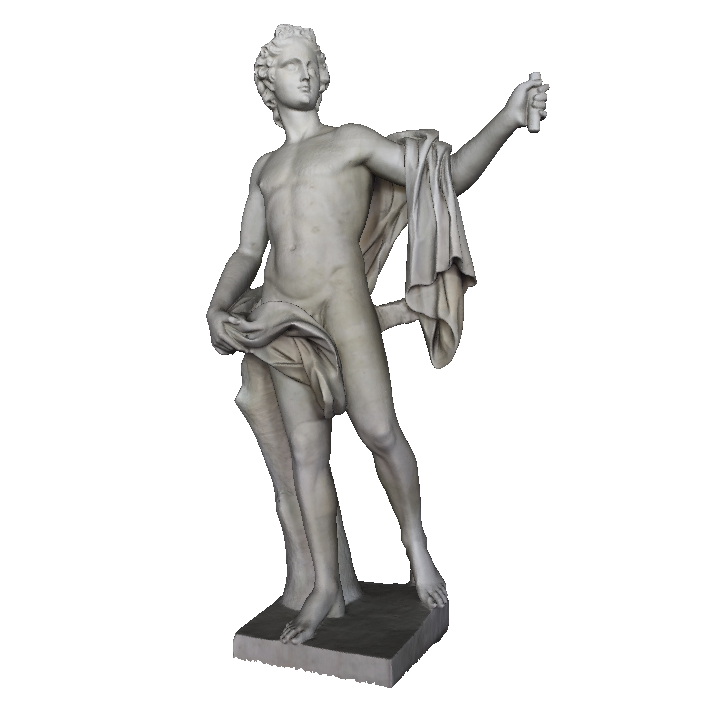
\includegraphics[width=\linewidth]{./Figures/train-dataset/00.apoll.png}
		\caption{apoll}
	\end{subfigure}
	\begin{subfigure}[b]{0.23\linewidth}
		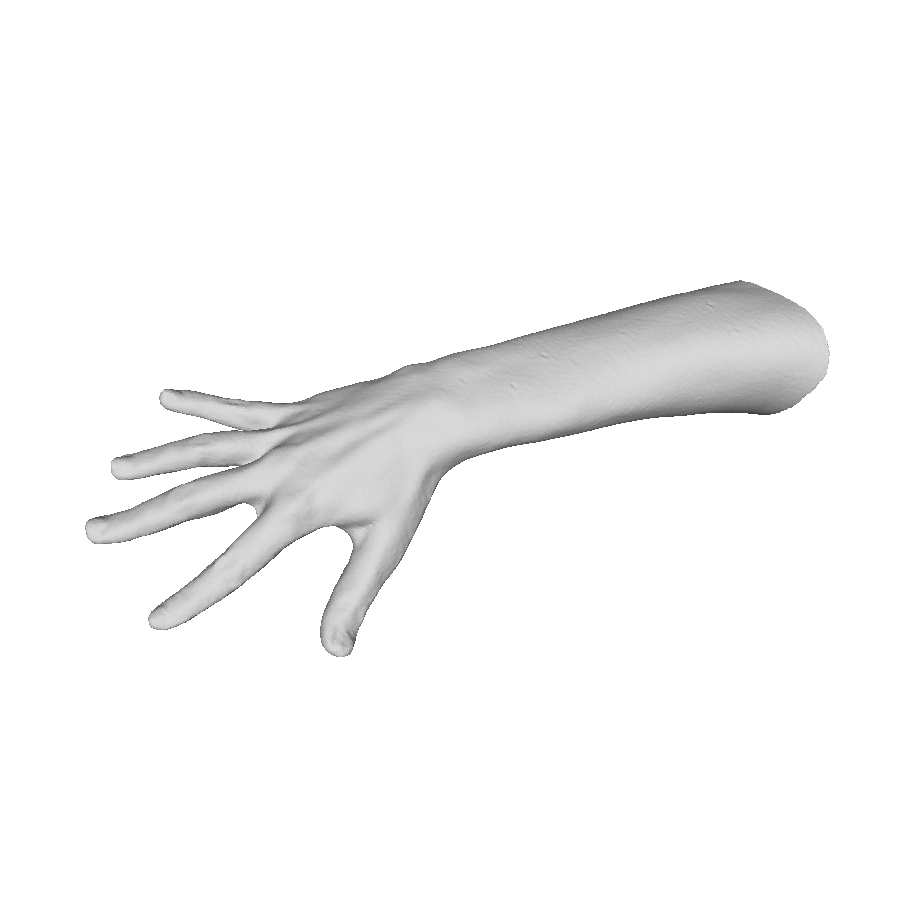
\includegraphics[width=\linewidth]{./Figures/train-dataset/01.arm.png}
		\caption{arm}
	\end{subfigure}
	\begin{subfigure}[b]{0.23\linewidth}
		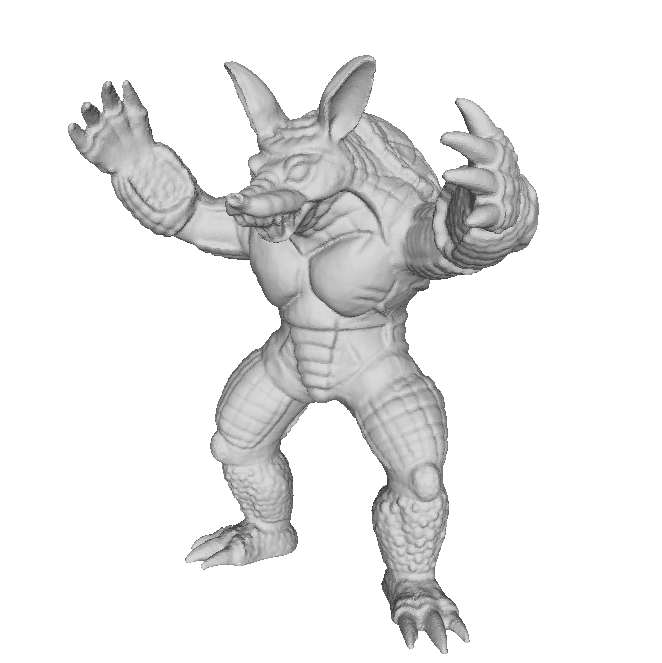
\includegraphics[width=\linewidth]{./Figures/train-dataset/02.armadillo.png}
		\caption{armadillo}
	\end{subfigure}
	\begin{subfigure}[b]{0.23\linewidth}
		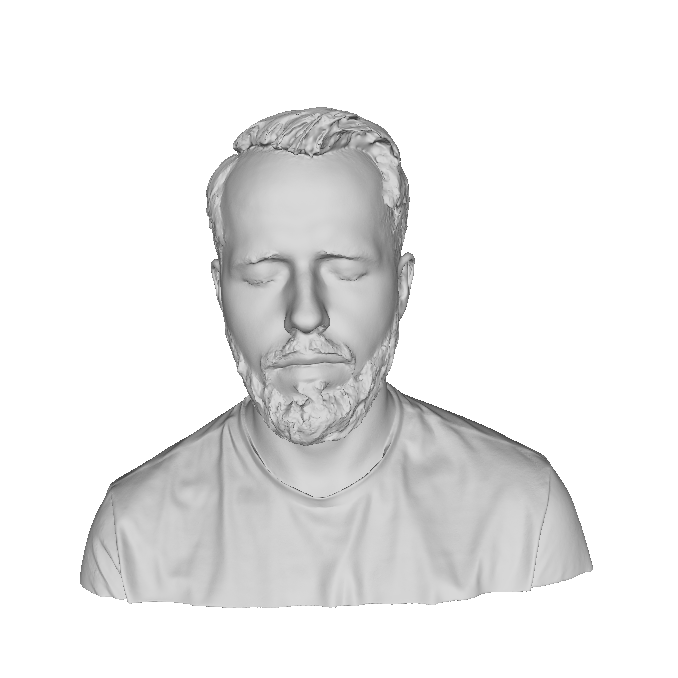
\includegraphics[width=\linewidth]{./Figures/train-dataset/03.bearded-guy.png}
		\caption{bearded-guy}
	\end{subfigure}
	
	\begin{subfigure}[b]{0.23\linewidth}
		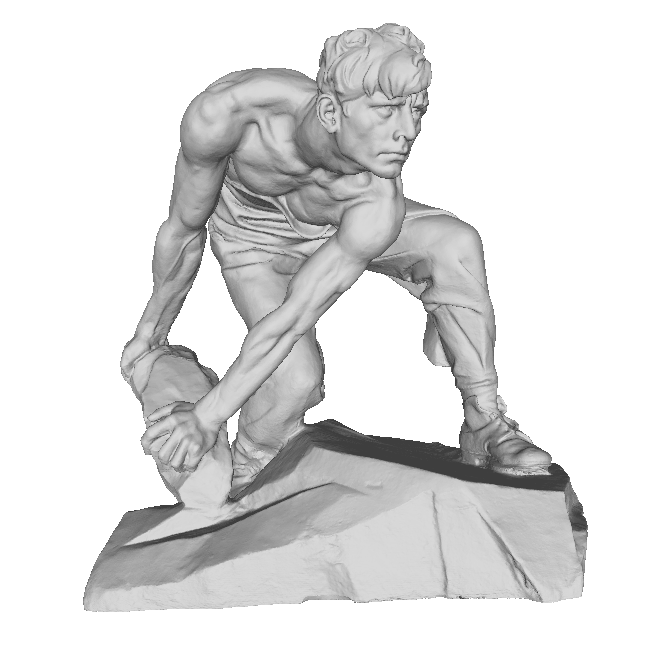
\includegraphics[width=\linewidth]{./Figures/train-dataset/04.bronze-sculpture.png}
		\caption{bronze-sculpture}
	\end{subfigure}
	\begin{subfigure}[b]{0.23\linewidth}
		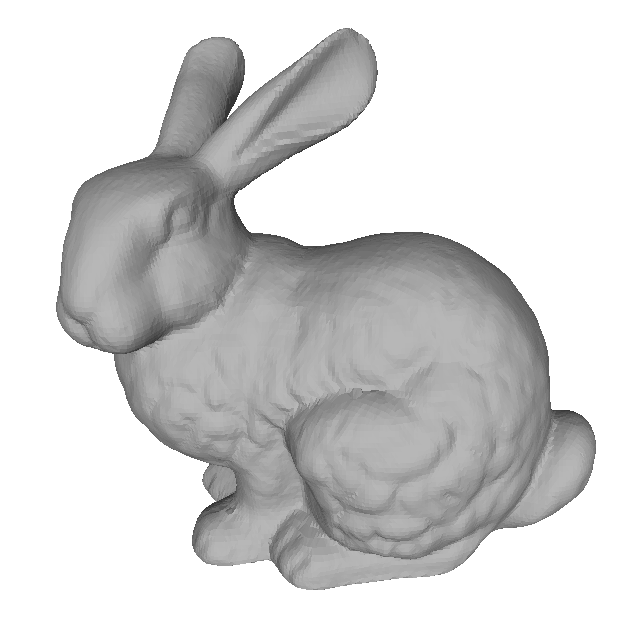
\includegraphics[width=\linewidth]{./Figures/train-dataset/05.bunny.png}
		\caption{bunny}
	\end{subfigure}
	\begin{subfigure}[b]{0.23\linewidth}
		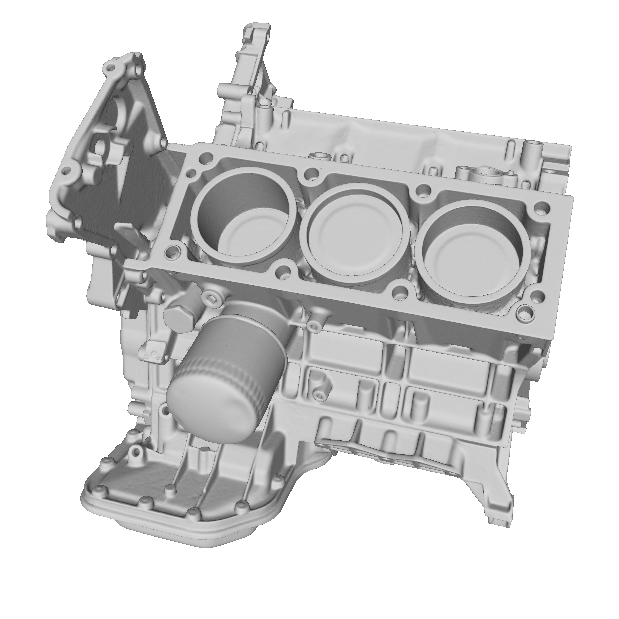
\includegraphics[width=\linewidth]{./Figures/train-dataset/06.car-engine.png}
		\caption{car-engine}
	\end{subfigure}
	\begin{subfigure}[b]{0.23\linewidth}
		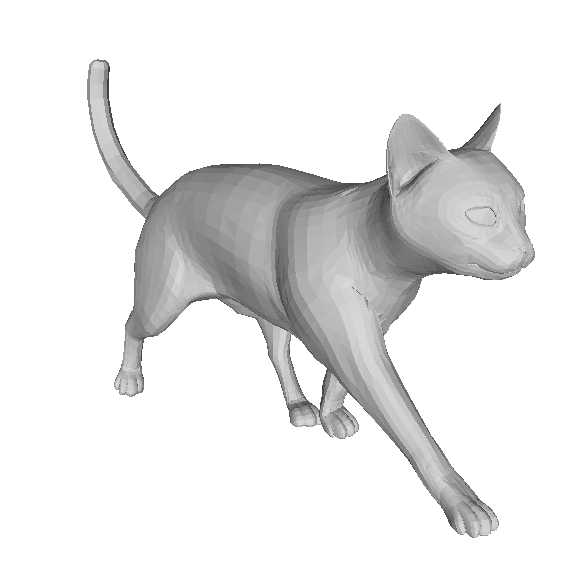
\includegraphics[width=\linewidth]{./Figures/train-dataset/07.cat.png}
		\caption{cat}
	\end{subfigure}
	
	\label{fig:dataset-demo}
	\caption{Point clouds scanned by high resolution scanners}
\end{figure}


\subsection{Synthesize Scenes using Unity}
In order to fit the using scenario of Kinect as much as possible, the dataset consists of the generated synthetic 3D scenes via Unity, which is a game engine using for 3D games creation. 

In the synthetic scenes from engine, the object is placed on a cylinder platform, which is lighted by a directional light nearby. A camera focus on the platform and captured the scene. The layout in the game engine is shown in Figure \ref{fig:unity-workplace}. In order to simulate more scenarios, the positions of the camera and directional light are randomly changed in each new scene. For 50 training objects, 1000 scenes are generated and each scene is saved in 3 kinds of resolutions $ 512\times512\times3 $, $ 256\times256\times3 $ and $ 128\times128\times3 $.

\begin{figure}[h!]
	\centering
	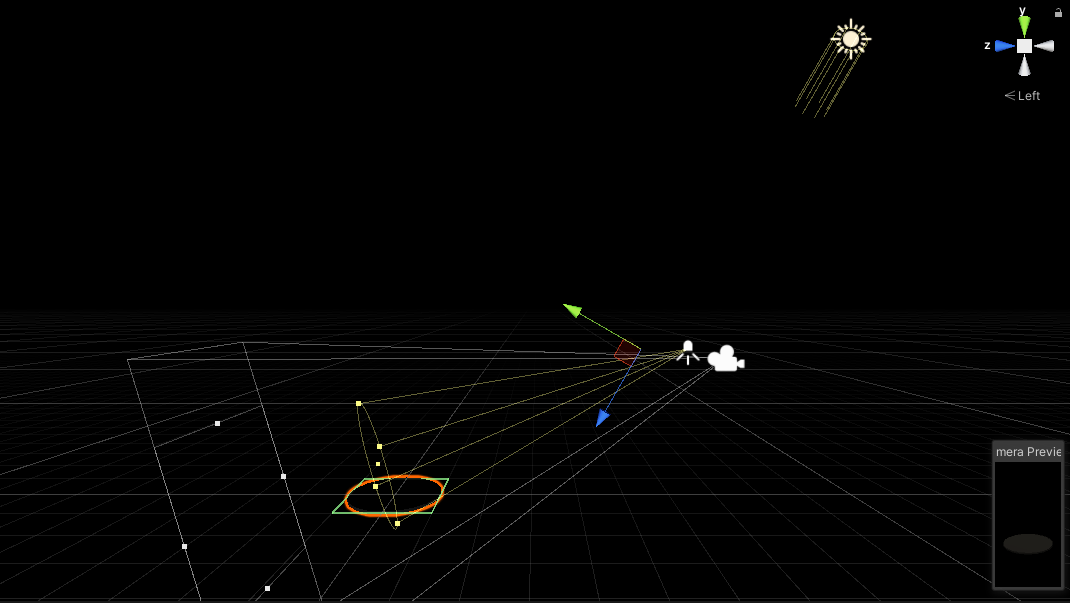
\includegraphics[width=.8\textwidth]{./Figures/unity-workplace.PNG}
	\caption{The layout of synthetic scenes generation in Unity.}
	\label{fig:unity-workplace}
\end{figure}

The main advantage using generated scene is the availability of complete information. The depth map can be captured in a loss-free way. The corresponding normal map can also be safely considered as ground truth. And the scale of the dataset is easy to control.

For each scene, following information is recorded
\begin{table}
	\caption{The information saved for each scene in ``synthetic50-5".}
	\label{tab:data-files}
	\centering
	\begin{tabular}{l l}
		\toprule
		\tabhead{Data} & \tabhead{Size} \\
		\midrule
		Depth map & $ 512\times512\times3 $ \\
		\hline 
		Depth range  & $ 2\times1 $ \\  
		\hline
		Grayscale Image	& $ 512\times512\times1 $ \\  
		\hline 
		Normal Map &  $ 512\times512\times3 $  \\
		\hline 
		Light Position &  $ 3\times1 $  \\
		\hline
		Camera Intrinsic Matrix &  $ 3\times 3 $  \\
		\hline 
		Camera Extrinsic Matrix &  $ 3\times 4 $  \\
		\hline 
		\bottomrule\\
	\end{tabular}
\end{table}

A depth map $ D $ is captured by a depth camera in Unity, which is a 1 channel image that contains the information relating to the distance of the surfaces of the scene objects from a viewpoint. It can be saved as a 16-bit grayscale image, i.e. each pixel in range $0 - 65535$. The grayscale image can be used as guided normal inference task and also as a readable scene for human. The gray-color is converted from RGB color based on following equation 
\[ gray: \frac{r+2g+b}{4}  \]
The normal map is the tangent surface normal, which is saved in 32-bit RGB color image. The surface normal $ (n_x, n_y, n_z) $ and its corresponding RGB color $ (R,G,B) $ can be converted based on following equation:
\begin{dgroup*}
	\begin{dmath*}
		n_x = \frac{R}{255} * 2 - 1
	\end{dmath*}
	\begin{dmath*}
		n_y = \frac{G}{255}*2 - 1
	\end{dmath*} 
	\begin{dmath*}
		n_z = 1-\frac{B}{255} * 2
	\end{dmath*}
\end{dgroup*}
If consider the relation between Lambertian reflection and normal direction, the light source can be used to calculate the reflect direction of each point.
The camera intrinsic and extrinsic matrix helps point cloud calculation.

It is necessary to point out again that ``synthetic50-5" aiming to rebuild the using scenarios of Kinect, where all types of the generated data files shown in Table \ref{tab:data-files} are also the same format of the Kinect data.



\subsection{Convert to Point Cloud}
\label{sec:depth-map-to-point-cloud}
The depth map can be converted to 3D vertex point cloud as the input of the normal inference model. 

\begin{figure}[h!]
	\centering
	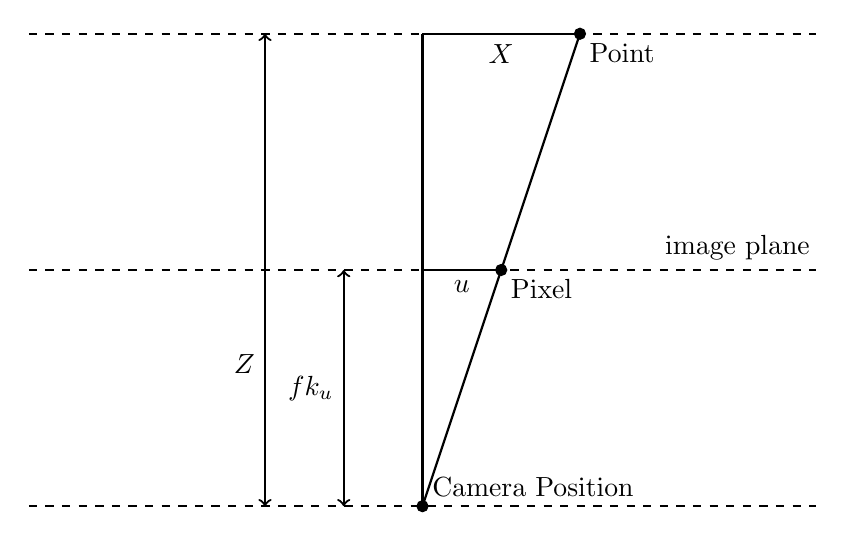
\begin{tikzpicture} 
		% reference lines
		\draw[thick,dashed]	(0,0) -- (10,0) ; % bottom
		\draw[thick,dashed]	(0,3) -- (10,3) node[pos=0.9, above] {image plane}; % middle
		\draw[thick,dashed]	(0,6) -- (10,6); % top
		% camera 
		\filldraw[black] (5,0) circle (2pt) node[anchor=south west]{Camera Position};
		% world point 
		\filldraw[black] (7,6) circle (2pt) node[anchor=north west]{Point};
		% image point
		\filldraw[black] (6,3) circle (2pt) node[anchor=north west]{Pixel};
		% similiar triangles
		\draw[thick] (5,0) -- (5,6); % AB
		\draw[thick] (5,0) -- (7,6); % AC
		\draw[thick] (5,6) -- (7,6) node[midway, below] {$ X $}; % BC
		\draw[thick] (5,3) -- (6,3) node[midway, below] {$ u $};
		% measure arrows
		\draw[thick, <->] (4,0) -- (4,3) node[midway, left] {$ fk_u $};
		\draw[thick, <->] (3,0) -- (3,6) node[pos=0.3, left] {$ Z $};
	\end{tikzpicture}	
	\caption{Convert depth to point in camera coordinate system}
	\label{fig:depth-triangulation}
\end{figure}

Consider a 3-dimensional Euclidean space. Use $ z $ axis denotes the depth. The $ x  $ and $ y $ axes perpendicular with each other. For a pixel $ (u,v) $ on depth map, its depth $ D(u,v) $ is the $ Z $ component of the corresponding point $P_C = (X,Y,Z) $ in camera coordinate system. The $ X $ and $ Y $ can be calculated based on the triangle similarity
\begin{dgroup*}
	
	\begin{dmath*}
		X = \frac{uZ}{fk_u}
	\end{dmath*}
	\begin{dmath*}
		Y = \frac{vZ}{fk_v}
	\end{dmath*}
\end{dgroup*}

where $ fk_u, fk_v $ is the focal length in pixels align $ u $ and $ v $ axes.
Converted a point from camera coordinate system to world coordinate system, using extrinsic matrix $ R $ and $ t $
\[P_W = P_CR+t \]

\subsection{Point Cloud Normalization}
\label{sec:dataset-normalization}
%% How to represent input tensor, to make it fast converse
The sizes of each training object are various, whereas it should be as an invariant value for the training model. Thus the normalization is required before feed training objects into the models.
The range of each axis is shown in Figure \ref{fig:data-range}.  Table \ref{tab:data-range} gives a quantitative measurement of corresponding average values. 

The normalization has been performed as follows. First translate the points to the original point as close as possible, then choose the range value of one axis as a scale factor, normalize the points to unit vectors. The equation is shown as follows
\begin{dgroup*}
	
	\begin{dmath*}
		X_n =\frac{X-\min(X)}{s}
	\end{dmath*}
	\begin{dmath*}
		Y_n = \frac{Y-\min(Y)}{s}
	\end{dmath*}
	
	\begin{dmath*}
		Z_n = \frac{Z-\min(Z)}{s}
	\end{dmath*}
\end{dgroup*}

where $ s $ is a scale factor, 

\begin{dmath*}
	s = \max(X)-\min(X)
\end{dmath*}
It is calculated as the range in $ X $ axis, but theoretically can be used by $ Y $ or $ Z $ axes as well.

\begin{figure}[!h]
	\centering
	{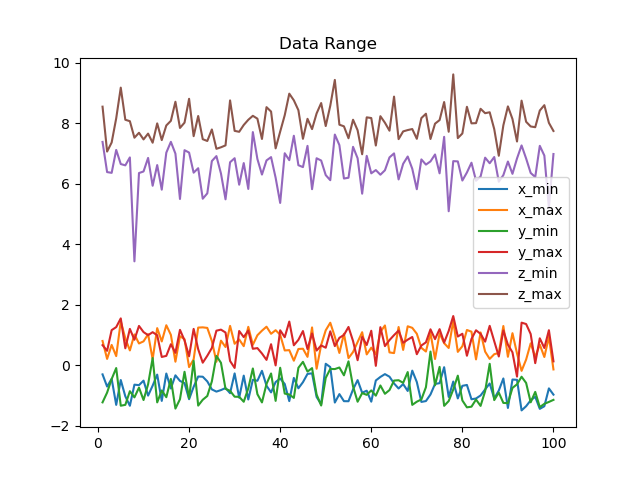
\includegraphics[width=0.45\textwidth]{./Figures/Data_Extreme.png}}
	{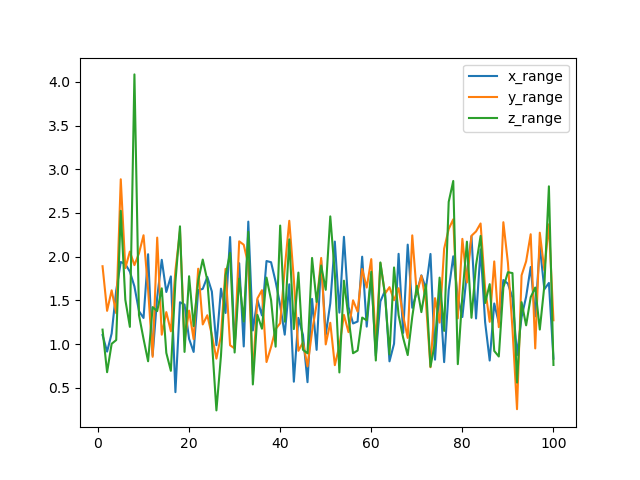
\includegraphics[width=0.45\textwidth]{./Figures/Data_Range.png}}
	\label{fig:data_range}
	\caption{Left: Extreme value in 3 axis; Right: Vertex range in 3 axis}
\end{figure}

\begin{table}[h!]
	\caption{ The fluctuation of extreme values and their ranges in 100 random training items. 
	}
	\label{tab:data-range}
	\centering
	\begin{tabular}{c c c c}
		\toprule
		\tabhead{Axis} & \tabhead{Scale} & \tabhead{Min} & \tabhead{Max}\\
		\midrule
		X & 1.48 & -0.75 & 0.73\\
		Y & 1.56 & -0.76 & 0.80\\
		Z & 1.47 & 6.53 & 8.00\\
		\bottomrule\\
	\end{tabular}
\end{table}



\subsection{Noise}
\label{sec:noise}
The raw depth maps captured by Kinect usually have missing pixels. Therefore, the ``synthetic50-5" dataset adds a similar properties.
As shown in Figure \ref{fig:depth_map_kinect}. the depth map has missing pixels distributed all around the scene.  Correspondingly, an uniformly distributed pixel-delete noise is used for noise simulation. 
Furthermore, a parameter $ \mu $ is used to control the intensity of noise, it denotes the $ \mu $-percent pixel dropoff. For example, $ \mu-10 $ means removes 10\% pixels randomly. For each scene, the noising operation based on a random $ \mu $ in a range $ \left[0, 50\right] $, therefore some scenes have more missing pixels and some have less. The random noise intensity also enables the model to learn scenarios not only with noise, but also with minor noise or even without noise.
Figure \ref{fig:noise-intensity} shows the noise effect on different $ \mu $.
%% add noise image
\begin{figure}[!h]
	\centering
	{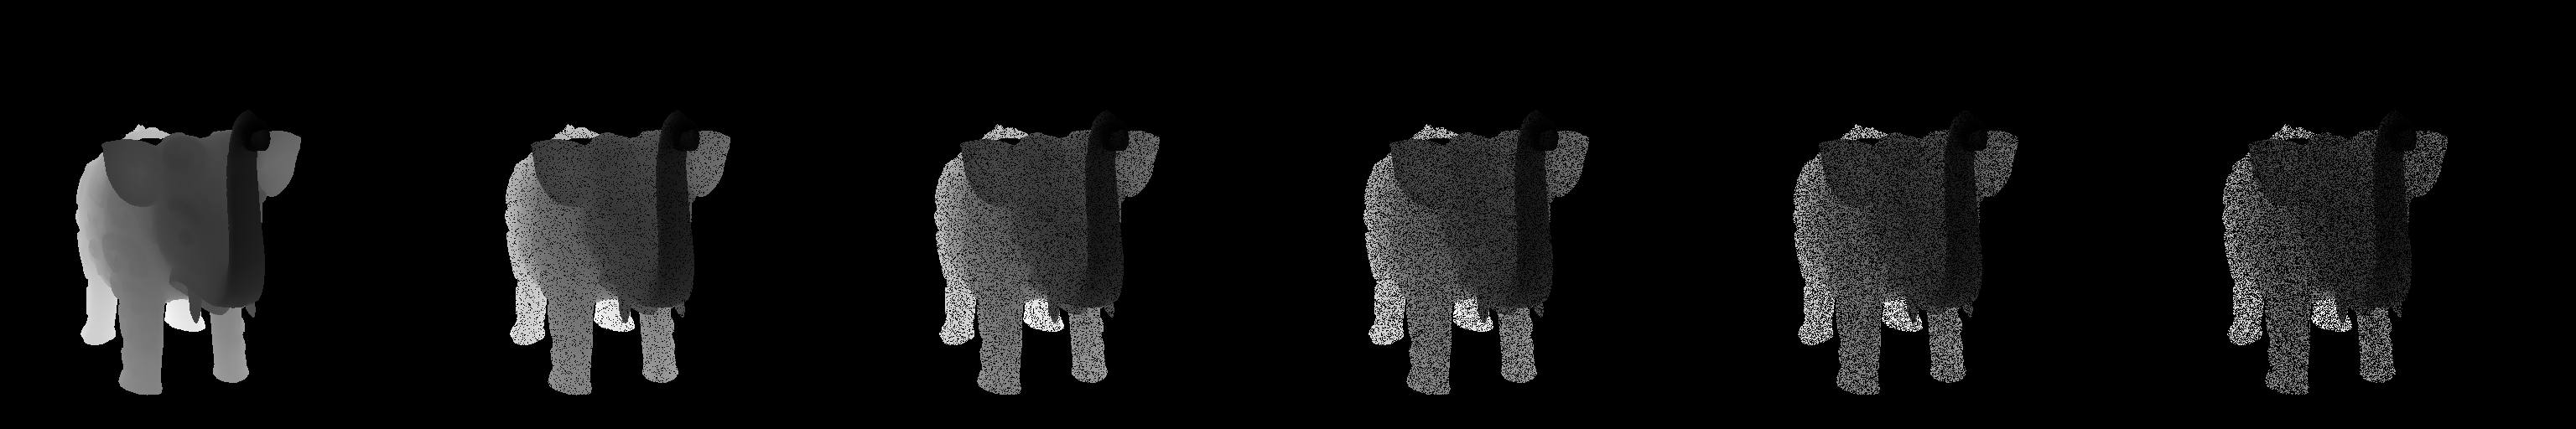
\includegraphics[width=.9\textwidth]{./Figures/add_noise_depth.png}}
	\decoRule	
	\caption{Noise-intensity on $ \mu-0, \mu-10,\mu-20, \mu-30, \mu-40, \mu-50,$. Object Name: elephant-zun-lid.}
	\label{fig:noise-intensity}
\end{figure}


\subsection{Fit to PyTorch}
In order to saving the training time, the dataset is compressed in PyTorch format. The structure of a single item is shown in Table \ref{tab:tensor-structure}.
\begin{table}
	\caption{The structure of a single tensor in the dataset.}
	\label{tab:tensor-structure}
	\centering
	\begin{tabular}{l l}
		\toprule
		\tabhead{Name} & \tabhead{Content} \\
		\midrule
		\multirow{3}{*}{input-tensor}  & Vertex \\  & Image \\  & Light Direction \\
		\hline
		\multirow{3}{*}{output-tensor}  & GT-Normal \\ & Image \\ & GT-Light-Direction \\
		\hline
		Light position & light position \\
		\hline 
		Camera Matrix  & K,R,t\\
		\hline 
		Depth Range  & minDepth, maxDepth\\
		\bottomrule\\
	\end{tabular}
\end{table}




\section{Real Dataset}

The real dataset is the depth map and rgb image captured via Kinect...

